\documentclass[9pt, a4paper]{arbeitsblatt}

\ladeModule{theme,tabellen,boxen}
\ladeFach[]{Informatik}

\aboptionen{
	name		= {J. Neugebauer},
	kuerzel		= {Ngb},
	titel		= {Vererbung},
	reihe		= {Objektorientierte Programmierung},
	fach		= {Informatik},
	lerngruppe	= {Q1},
	nummer		= {I.07},
	lizenz		= {cc-by-nc-sa-4},
	version		= {2022-09-15},
}

\begin{document}
\ReiheTitel

Fork und klone das Projekt \ordner{Medienplayer\_Entwurf3} vom Git-Server.
\begin{enumn}
	\item\label{ta-eins} Studiert und testet zunächst nur die Klasse \code{Video}, insbesondere die Methode \code{ausgabe()}\footnote{Die Methode \code{ausgabe()} ist nicht Teil des Klassendiagramms und wurde nachträgliche ergänzt.}. Was fällt euch auf? Was ist ungewöhnlich oder neu für euch? \textit{Markiert Besonderheiten mit Kommentaren im Quelltext.}

	\item Zieht nun auch die Klasse \code{Mediendatei} hinzu. Könnt ihr einige der Besonderheiten aus \ref{ta-eins} erklären? Notiert euch Stichpunkte.
\end{enumn}
\begin{rahmen}
\begin{tabularx}{\linewidth}{|c|X|p{6cm}}
	\multicolumn{2}{l}{Erkläre folgende Begriffe / Schlüsselworte:} & Klassendiagramm: \\ \cline{1-2}
	Oberklasse (Superclass) & \Zeilenabstand & \\ \cline{1-2}
	Unterklasse (Subclass) & \Zeilenabstand & \\ \cline{1-2}
	\code{extends} & \Zeilenabstand & \\ \cline{1-2}
	\code{protected} & \Zeilenabstand & \\ \cline{1-2}
	\code{abstract} & \Zeilenabstand & \\ \cline{1-2}
	\code{super} & \Zeilenabstand & \\ \cline{1-2}
\end{tabularx}
\end{rahmen}
\begin{enumn}[resume*]
	\item Implementiert anhand des Beispiels der Klasse \code{Video} die Klasse \code{Audio} oder \code{Bild} passend zum Implementierungsdiagramm unten.
\end{enumn}
\begin{center}
	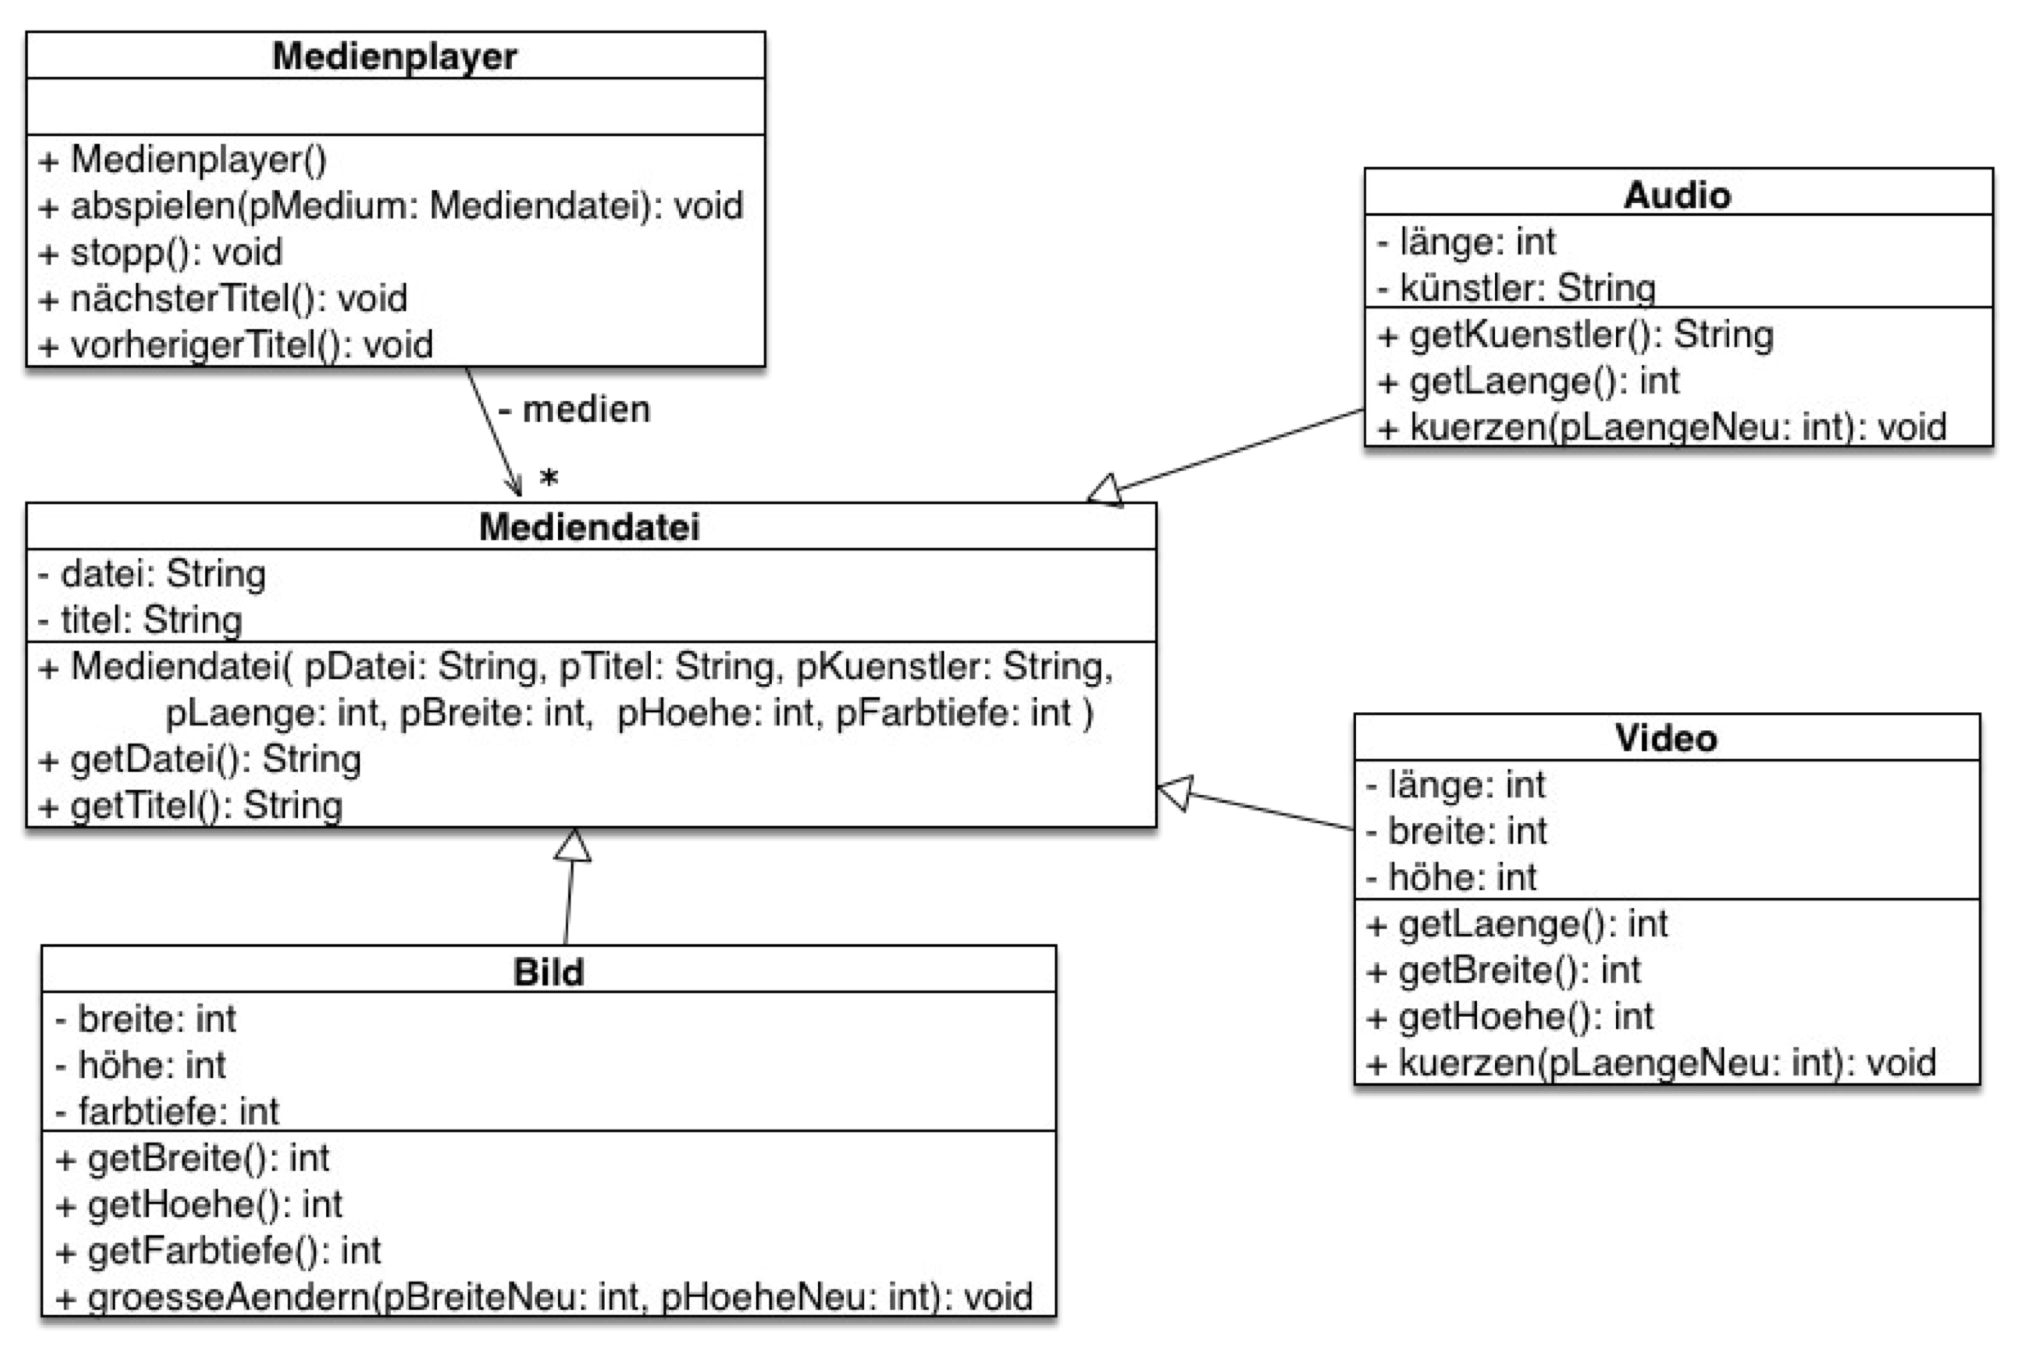
\includegraphics[height=8cm]{Q1-AB.I.07-Abb_Medienplayer_UML.png}
\end{center}
%\subsubsection*{Zusatzaufgabe}
\begin{enumn}[resume*]
	\item \code{Video} und \code{Audio} haben beide das Attribut \code{Laenge} und die Methode \code{kuerzen()}.

	Implementiere eine neue Klasse \code{AbspielbareMediendatei}, die \emph{Unterklasse} von \code{Mediendatei} ist und \emph{Oberklasse} von \code{Audio} und \code{Video}.
\end{enumn}

\newpage
\emph{Unterklassen} können Methoden ihrer \emph{Oberklassen} \enquote{überschreiben}. Dazu implementiert eine Unterklasse eine Methode mit der exakten \emph{Signatur} der Methode in der Oberklasse. Eine \emph{Unterklasse} kann die Implementation der Oberklasse mit Hilfe des Schlüsselwortes \code{super} aufrufen.

\begin{enumn}[resume*]
	\item Fork und klone das Projekt \ordner{Karneval der Tiere} vom Git-Server. Analysiere den Code und studiere insbesondere die \code{sagWas} Methoden der verschiedenen Klassen. Erstelle auch Objekte der Tiere und lass sie etwas \enquote{sagen}.

	\begin{smallenum}
		\item Beschreibe das Konzept des Überschreibens von Methoden anhand des Karneval-Projektes.
		\item Ergänze mindestens drei weitere Tiere im Projekt. Orientiere dich an den gezeigten Klassen.
		\item Überschreibe die Methode \code{sagWas()} in den \emph{Unterklassen}.
		\item Implementiere die Methode \code{sagWas} in der Klasse \code{KarnevalDerTiere}.
		\item Ergänze neue \emph{Oberklassen}, die Tiere einer Art zusammenfassen (z.B: \enquote{Fliegend}, \enquote{Schwimmend}, \enquote{Laufend}, ...).
	\end{smallenum}
\end{enumn}

\end{document}
